Since the satellite consists of two rotational masses, the kinetic energy is the sum of the rotational kinetic energy of each mass.  Therefore the kinetic energy is given by
\begin{equation}\label{eq:satellite_kinetic_energy}
K = \frac{1}{2} J_s \dot{\theta}^2 + \frac{1}{2} J_p \dot{\phi}^2.
\end{equation}

Throughout the book, we will demonstrate how to simulate the satellite using
Python code.  The code that animates the satellite and implements the animation is given below.

%\lstinputlisting[language=Python, basicstyle=\ttfamily\scriptsize, breaklines=true, caption=satelliteAnimation.py]{../control_book_public_solutions/_C_satellite/python/hw2/satelliteAnimation.py}

\lstinputlisting[language=Python, caption=satelliteAnimation.py]{../control_book_public_solutions/_C_satellite/python/hw2/satelliteAnimation.py}

The Python code that implements the animation is given below.
\lstinputlisting[language=Python, caption=satelliteSim.py]{../control_book_public_solutions/_C_satellite/python/hw2/satelliteSim.py}


%\begin{figure}[hbt]
%	\begin{subfigure}{.5\textwidth}
%  	\centering
%  	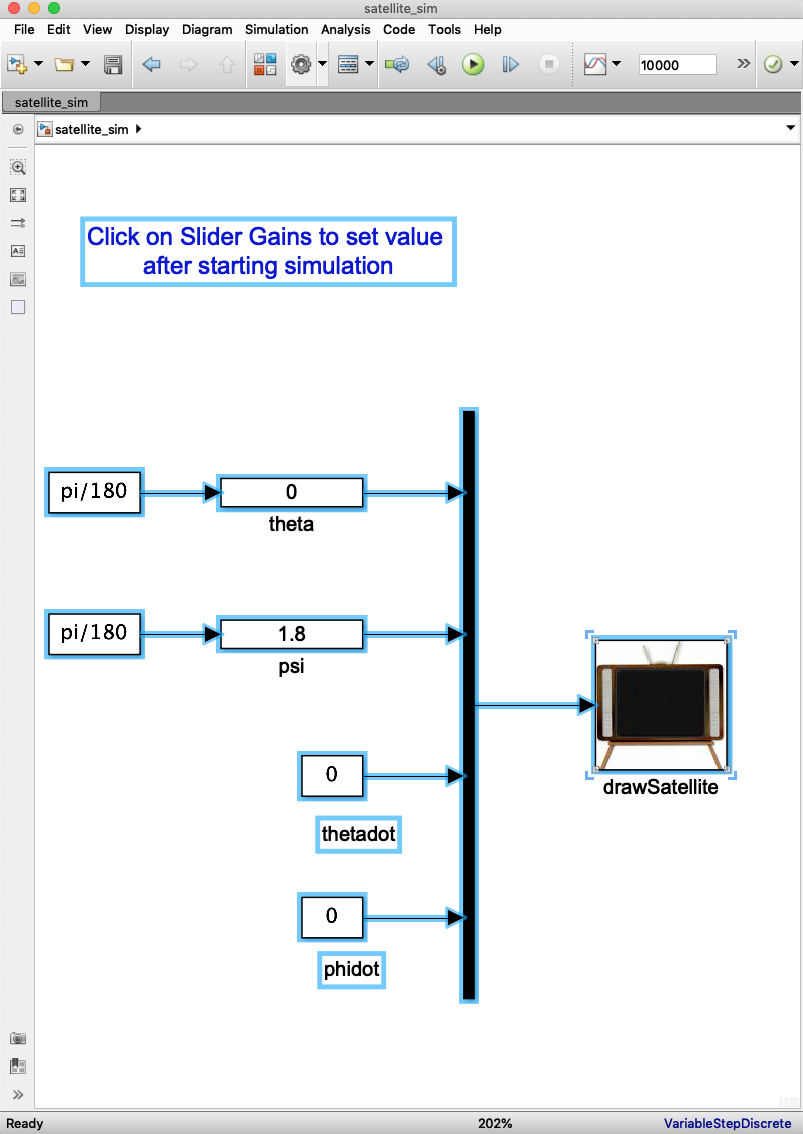
\includegraphics[width=.95\linewidth]{6_design_studies/_C_satellite/LaTeX/hw2/figures/satellite_sim_main}
  	%\caption{}
  	%\label{fig:sub1}
%	\end{subfigure}%
%	\begin{subfigure}{.5\textwidth}
%  	\centering
%  	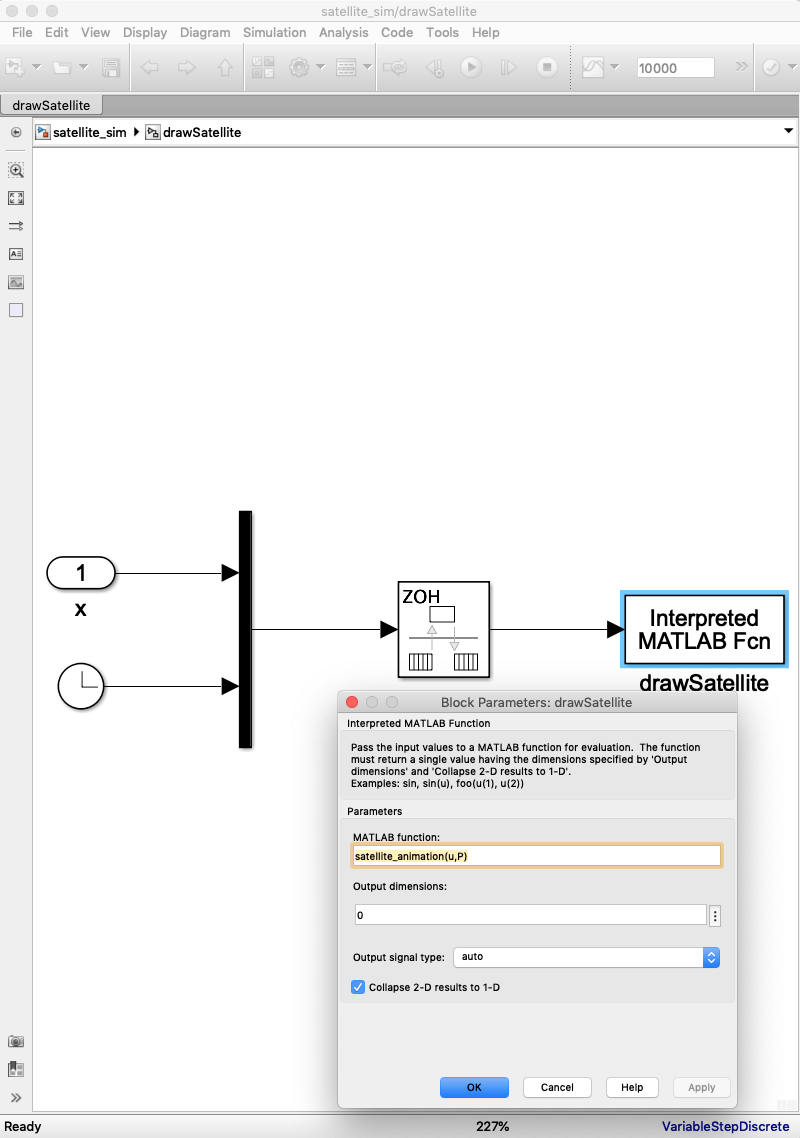
\includegraphics[width=.95\linewidth]{6_design_studies/_C_satellite/LaTeX/hw2/figures/satellite_sim_animation}
  	%\caption{A subfigure}
  	%\label{fig:sub2}
%	\end{subfigure}
%  \caption{Simulink diagrams for Satellite animation}
%  \label{fig:hw2_satellite_sim}  
%\end{figure}

Complete simulation code for Matlab, Python, and Simulink can be downloaded at \controlbookurl{http://controlbook.byu.edu}.





